\chapter{Implementation}
\label{sec:implementation}
The main idea of our implementation is to partition the grid into equal two-dimensional tiles of size $t_w \times t_h$ and assign each tile to a single \ac{pe}, with the benefit that most values required for computing the next iteration already reside in the same \acp{pe}. For the cells on the border-region of the tile, values from neighboring tiles are required. Since communication on Cerebras hardware is limited to the four direct neighbor elements, communication patters that require data to move between non-adjacent \acp{pe}, are far more complex to implement and come with significant communication overhead. For that reason, we limit the scope of this work to parameter combinations that require only communication with the direct neighboring \acp{pe}. This means that the radius of the stencil must be smaller or equal to the tile size, specifically
\begin{equation}    
\label{eq:radius_constraint}
r \leq \min(t_w, t_h)
\end{equation}

For the simple case where $t_w=t_h=1$, this results in a radius of 1.

Two main approaches were implemented:
\begin{itemize}
    \item A specialized, single cell implementation, that represents each element of the grid with one \ac{pe} and restricts the radius to one
    \item A general, tiled implementation maps multiple elements of the underlying grid, i.e., a tile size of $t_w \times t_h$, to a single \ac{pe}, allows for grid sizes that significantly exceed the \ac{wse} hardware dimensions and a radius greater than one as long as \autoref{eq:radius_constraint} is satisfied 
\end{itemize}

A special case of the tiled implementation, where the radius is one, has been further optimized to reduce overhead. We refer to this as the r1-optimized version of the tiled implementation. 

Although the experiments throughout this thesis utilize symmetric, constant coefficients, the presented implementations offer different degrees of flexibility for more general stencil forms.

The single cell implementation, as well as the r1-optimized tiled version, leverage optimizations that rely on symmetric coefficients. This restriction enables significant performance gains for this specific use case. In contrast, the general tiled implementation could handle asymmetric coefficients with minimal modifications without increasing the number of computational cycles.

Regarding spatially varying coefficients, all implementations could be adapted to handle them without performance degradation. The tiled implementations are already designed for each PE to receive its own set of coefficients from the host, meaning a shift to variable coefficients would require no changes to the CSL kernel. The non-tiled implementation currently uses fixed weights but could support variable coefficients with a minor modification which would also incur no runtime overhead.

The tiled implementation consists of a top-level time-step loop comprising separate data exchange and compute steps in each iteration, while the single-cell implementation interleaves the two steps.

\begin{figure}
    \centering
    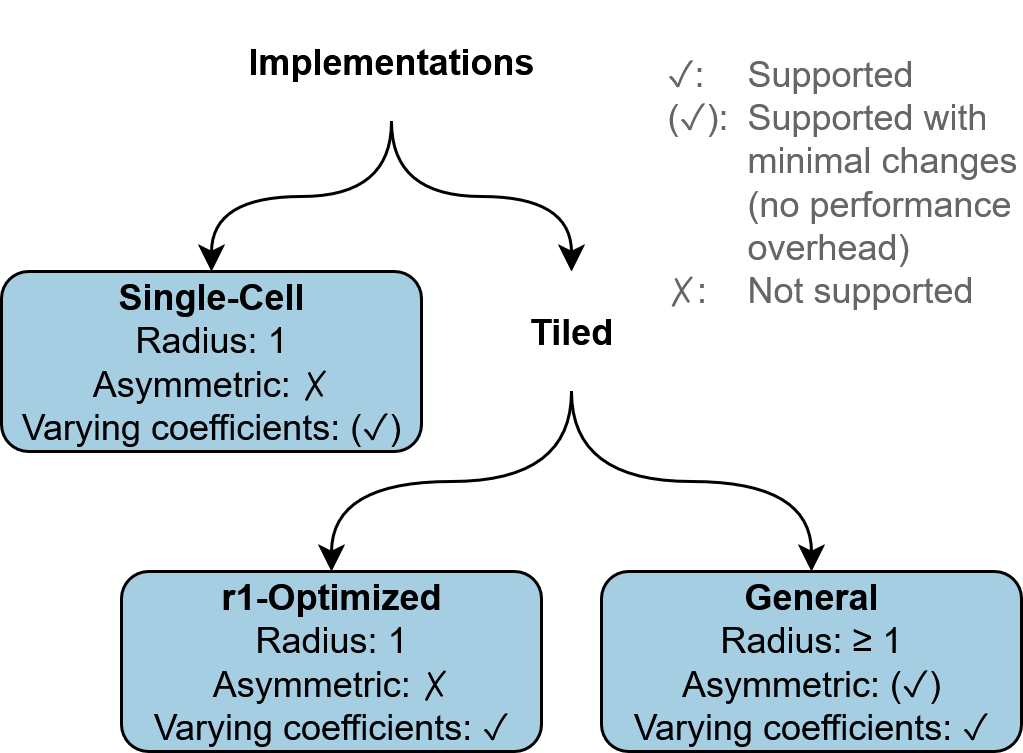
\includegraphics[width=0.5\linewidth]{implementations.png}
    \caption{Visualization of the implementations}
    \label{fig:implementations}
\end{figure}

\section{Single-cell implementation}
This specialization allows a heavily optimized implementation, but restricts the maximum problem size to the \ac{wse} hardware dimensions.
The computation for each element can be described as follows:
\begin{equation}
    \label{eq:stencil_computation}
    v^{'} = w_0 \cdot v + w_1 \cdot (v_{north} + v_{east} + v_{south} + v_{west})
\end{equation}
Where $v$ is the old value of the element, $v_{north}, v_{east}, v_{south}, v_{west}$ are the values of the four neighbors, $w_0, w_1$ are the stencil coefficients and $v^{'}$ is the new value of the element.

\subsection{Data exchange and routing configuration}
Each \ac{pe} sends data to, and receives data from its four direct neighboring \acp{pe}. Notably it sends the same data to the four neighbors. This allows for increased communication speed by using the build-in broadcasting functionality of the router. We assign each \ac{pe} a color and define a route so that the router receives data on this color from the \ac{ce} and sends it to the four neighboring routers, which are configured to forward the data to their respective \acp{ce}. Because only one route can be defined per color and router, we use a pattern containing six distinct colors to map the grid.
The coloring rule can be described as following function $f:\mathbb{N}\times\mathbb{N}\to\{0,1,2,3,4,5\}$:
\begin{equation}
    \label{eq:coloring_function}
    f(x,y) = (x + 2y) \bmod 6
\end{equation}
and visualized in \autoref{fig:r1_stencil_coloring}.
\begin{figure}
    \centering
    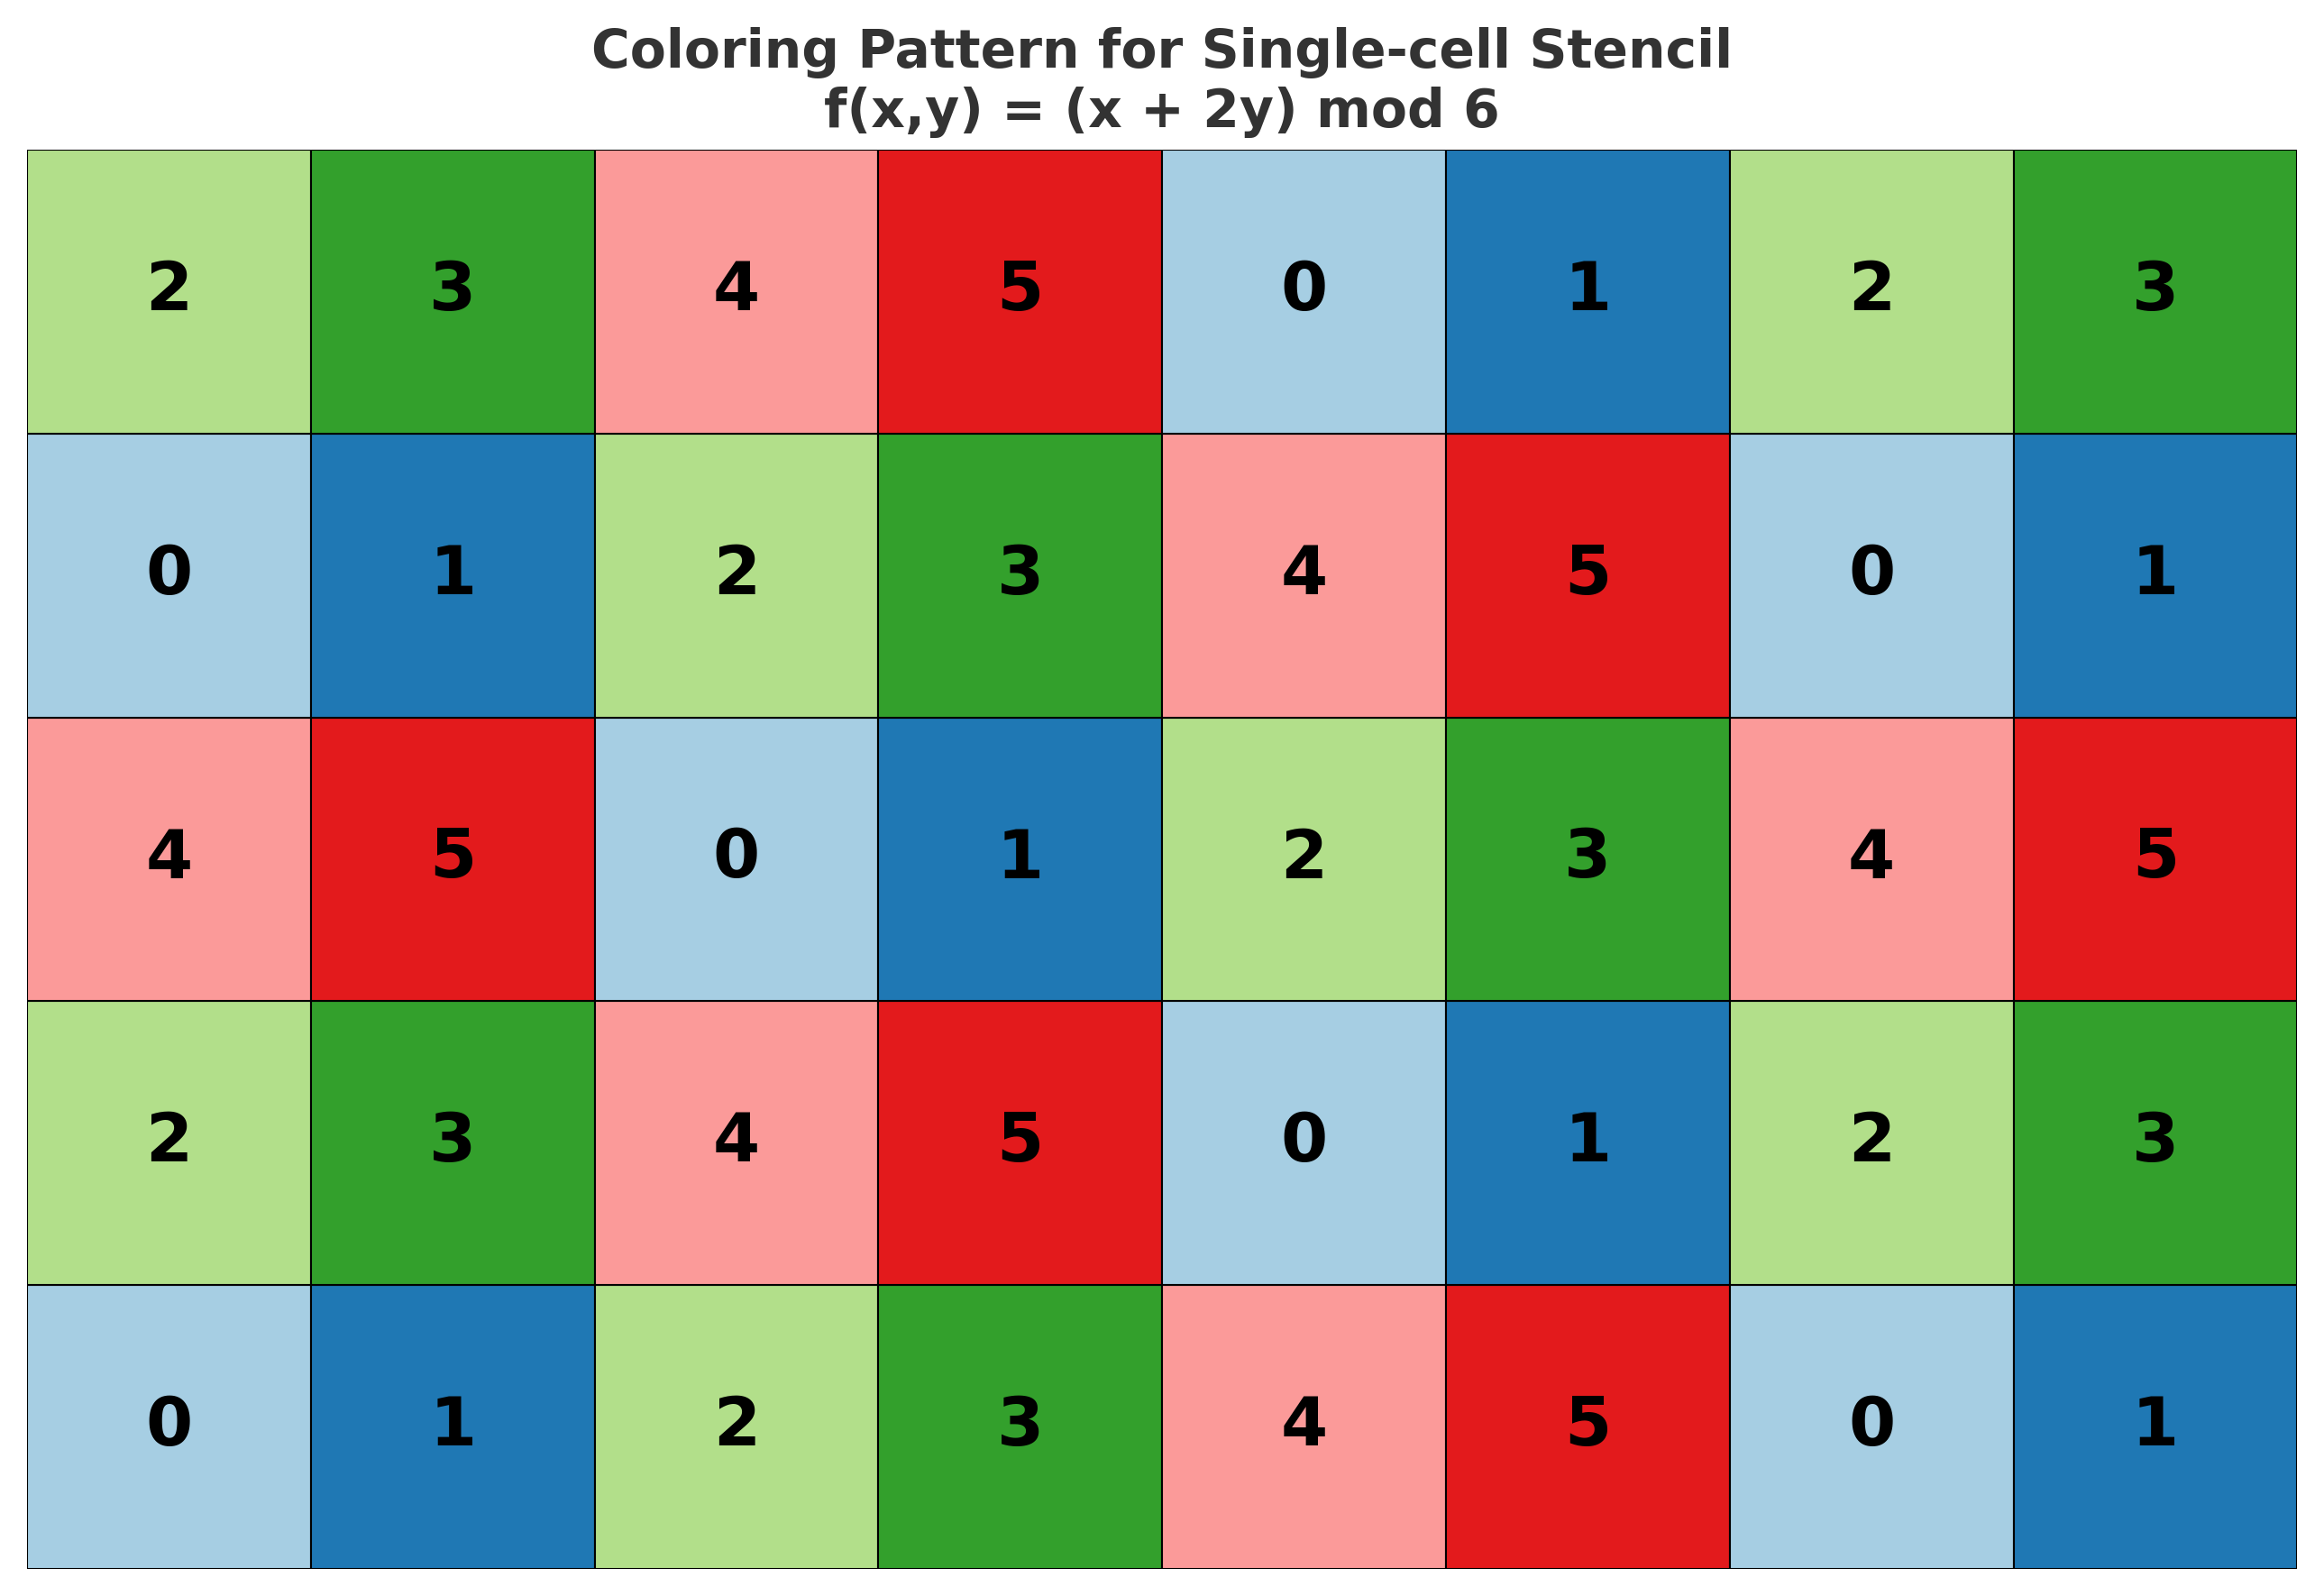
\includegraphics[width=0.5\linewidth]{r1-stencil-coloring.png}
    \caption{Visualization of the coloring pattern for radius-1 non-tiled stencil. Each color represents a distinct routing color (0-5) used for conflict-free communication between \acp{pe}. The numbers in each cell show the color index computed by $f(x,y) = (x + 2y) \bmod 6$}
    \label{fig:r1_stencil_coloring}
\end{figure}

\subsection{\ac{pe} Program}
The implementation for the radius-1, non-tiled case is relatively simple.
Although only single elements are processed at a time, \acp{dsd} are needed for communication and for performance reasons explicit \ac{dsr} assignment is employed, decreasing the number of cycles per iteration significantly.  
Further, the center multiplication is placed at the beginning of each iteration in a way that it overlaps with the communication delay and does not need an additional cycle.
Because only one fp32 element is received from and send to each neighbour, input and output queues never fill up completely and synchronous \ac{dsd} operations can be used instead of asynchronous operations that add significant overhead.
Furthermore, the algorithm multiplies the value which is send to the neighbors with the coefficient $w_1$ while sending, so that the receiving \acp{pe} only add these values to $w_0 \cdot v$ to get the new value.
By computing the intermediate values $intermediate_1$ and $intermediate_2$ before adding them to $value$, the number of cycles for this part of the calculation is reduced from 10 to 7.

% \begin{algorithm}[tbh]
%     \SetAlgoLined
%     \KwData{Received values from neighbors}
%     \KwResult{Updated value}
%     $intermediate_1 \gets \Call{ReceiveFromNorth}{} + \Call{ReceiveFromEast}{}$\;
%     $intermediate_2 \gets \Call{ReceiveFromSouth}{} + \Call{ReceiveFromWest}{}$\;
%     $value \gets value + intermediate_1$\;
%     $value \gets value + intermediate_2$\;
%     \caption{Algorithm with intermediate values}\label{alg:intermediate_values}
% \end{algorithm}

% use csl code instead of algorithm
\begin{lstlisting}[language=CSL, caption={CSL code for the single-cell implementation}, label={lst:single_cell_implementation}]
    if (@is_arch("wse2")){
        @fadds(intermediate_sum_1_dsr_dest, recv_dsr_east, recv_dsr_west);
        @fadds(intermediate_sum_2_dsr_dest, recv_dsr_north, recv_dsr_south);
        @fadds(cell_value_dsr, cell_value_dsr, intermediate_sum_1_dsr_src1);
        @fadds(cell_value_dsr, cell_value_dsr, intermediate_sum_2_dsr_src1);
      }else{
        // two fabric inputs not allowed on WSE-3
        @fadds(cell_value_dsr, cell_value_dsr, recv_dsr_east);
        @fadds(cell_value_dsr, cell_value_dsr, recv_dsr_west);
        @fadds(cell_value_dsr, cell_value_dsr, recv_dsr_north);
        @fadds(cell_value_dsr, cell_value_dsr, recv_dsr_south);
      }
\end{lstlisting}


While the reason for this performance benefit cannot be explained by the publicly available documentation from Cerebras, speculation from limited testing suggests that values seem to be available to a following operation only three cycles after they were written to.
Our empirical analysis revealed a data dependency stall: an operation using a register as an operand is delayed until at least three cycles have passed since that register was last written to. While this behavior is not detailed in the public documentation, it consistently impacts performance. By reordering the computation to use intermediate variables (as shown in \autoref{alg:intermediate_values}), we mitigate these stalls, reducing the cycle count for this computational segment from 10 to 7 cycles.

Unfortunately, this does not work on WSE-3, since it allows at most one fabric \ac{dsd} arguments per operation.

\begin{table}[h]
    \centering
    \caption{Operations for one grid point and iteration in the radius-1, non-tiled implementation}
    \label{tab:r1_non_tiled_operations}
    \begin{tabular}{@{}cccc@{}}
        \toprule
        Operation & Cerebras Op Code & Count & Flops \\
        \midrule
        add & \texttt{@fadds} & \num{4} & \num{4} \\
        mul & \texttt{@fmuls} & \num{2} & \num{2} \\
        \midrule
        total & & \num{6} & \num{6} \\
        \bottomrule
    \end{tabular}
\end{table}

\section{Tiled implementation}
For a radius greater or equal to one, the computation can be expressed as follows:
\begin{equation}
    \label{eq:stencil_computation_tiled}
    v^{'} = w_0 \cdot v + \sum_{i=1}^{r} w_i \cdot (v_{north,i} + v_{east,i} + v_{south,i} + v_{west,i})
\end{equation}
Where $v$ is the old value of the element, $v_{north,i}, v_{east,i}, v_{south,i}, v_{west,i}$ are the values of the four neighbors at distance $i$ from the center and $w_0, w_1, \dots, w_r$ are the symmetric stencil coefficients.

\subsection{Data exchange and routing configuration}
\begin{figure}
    \centering
    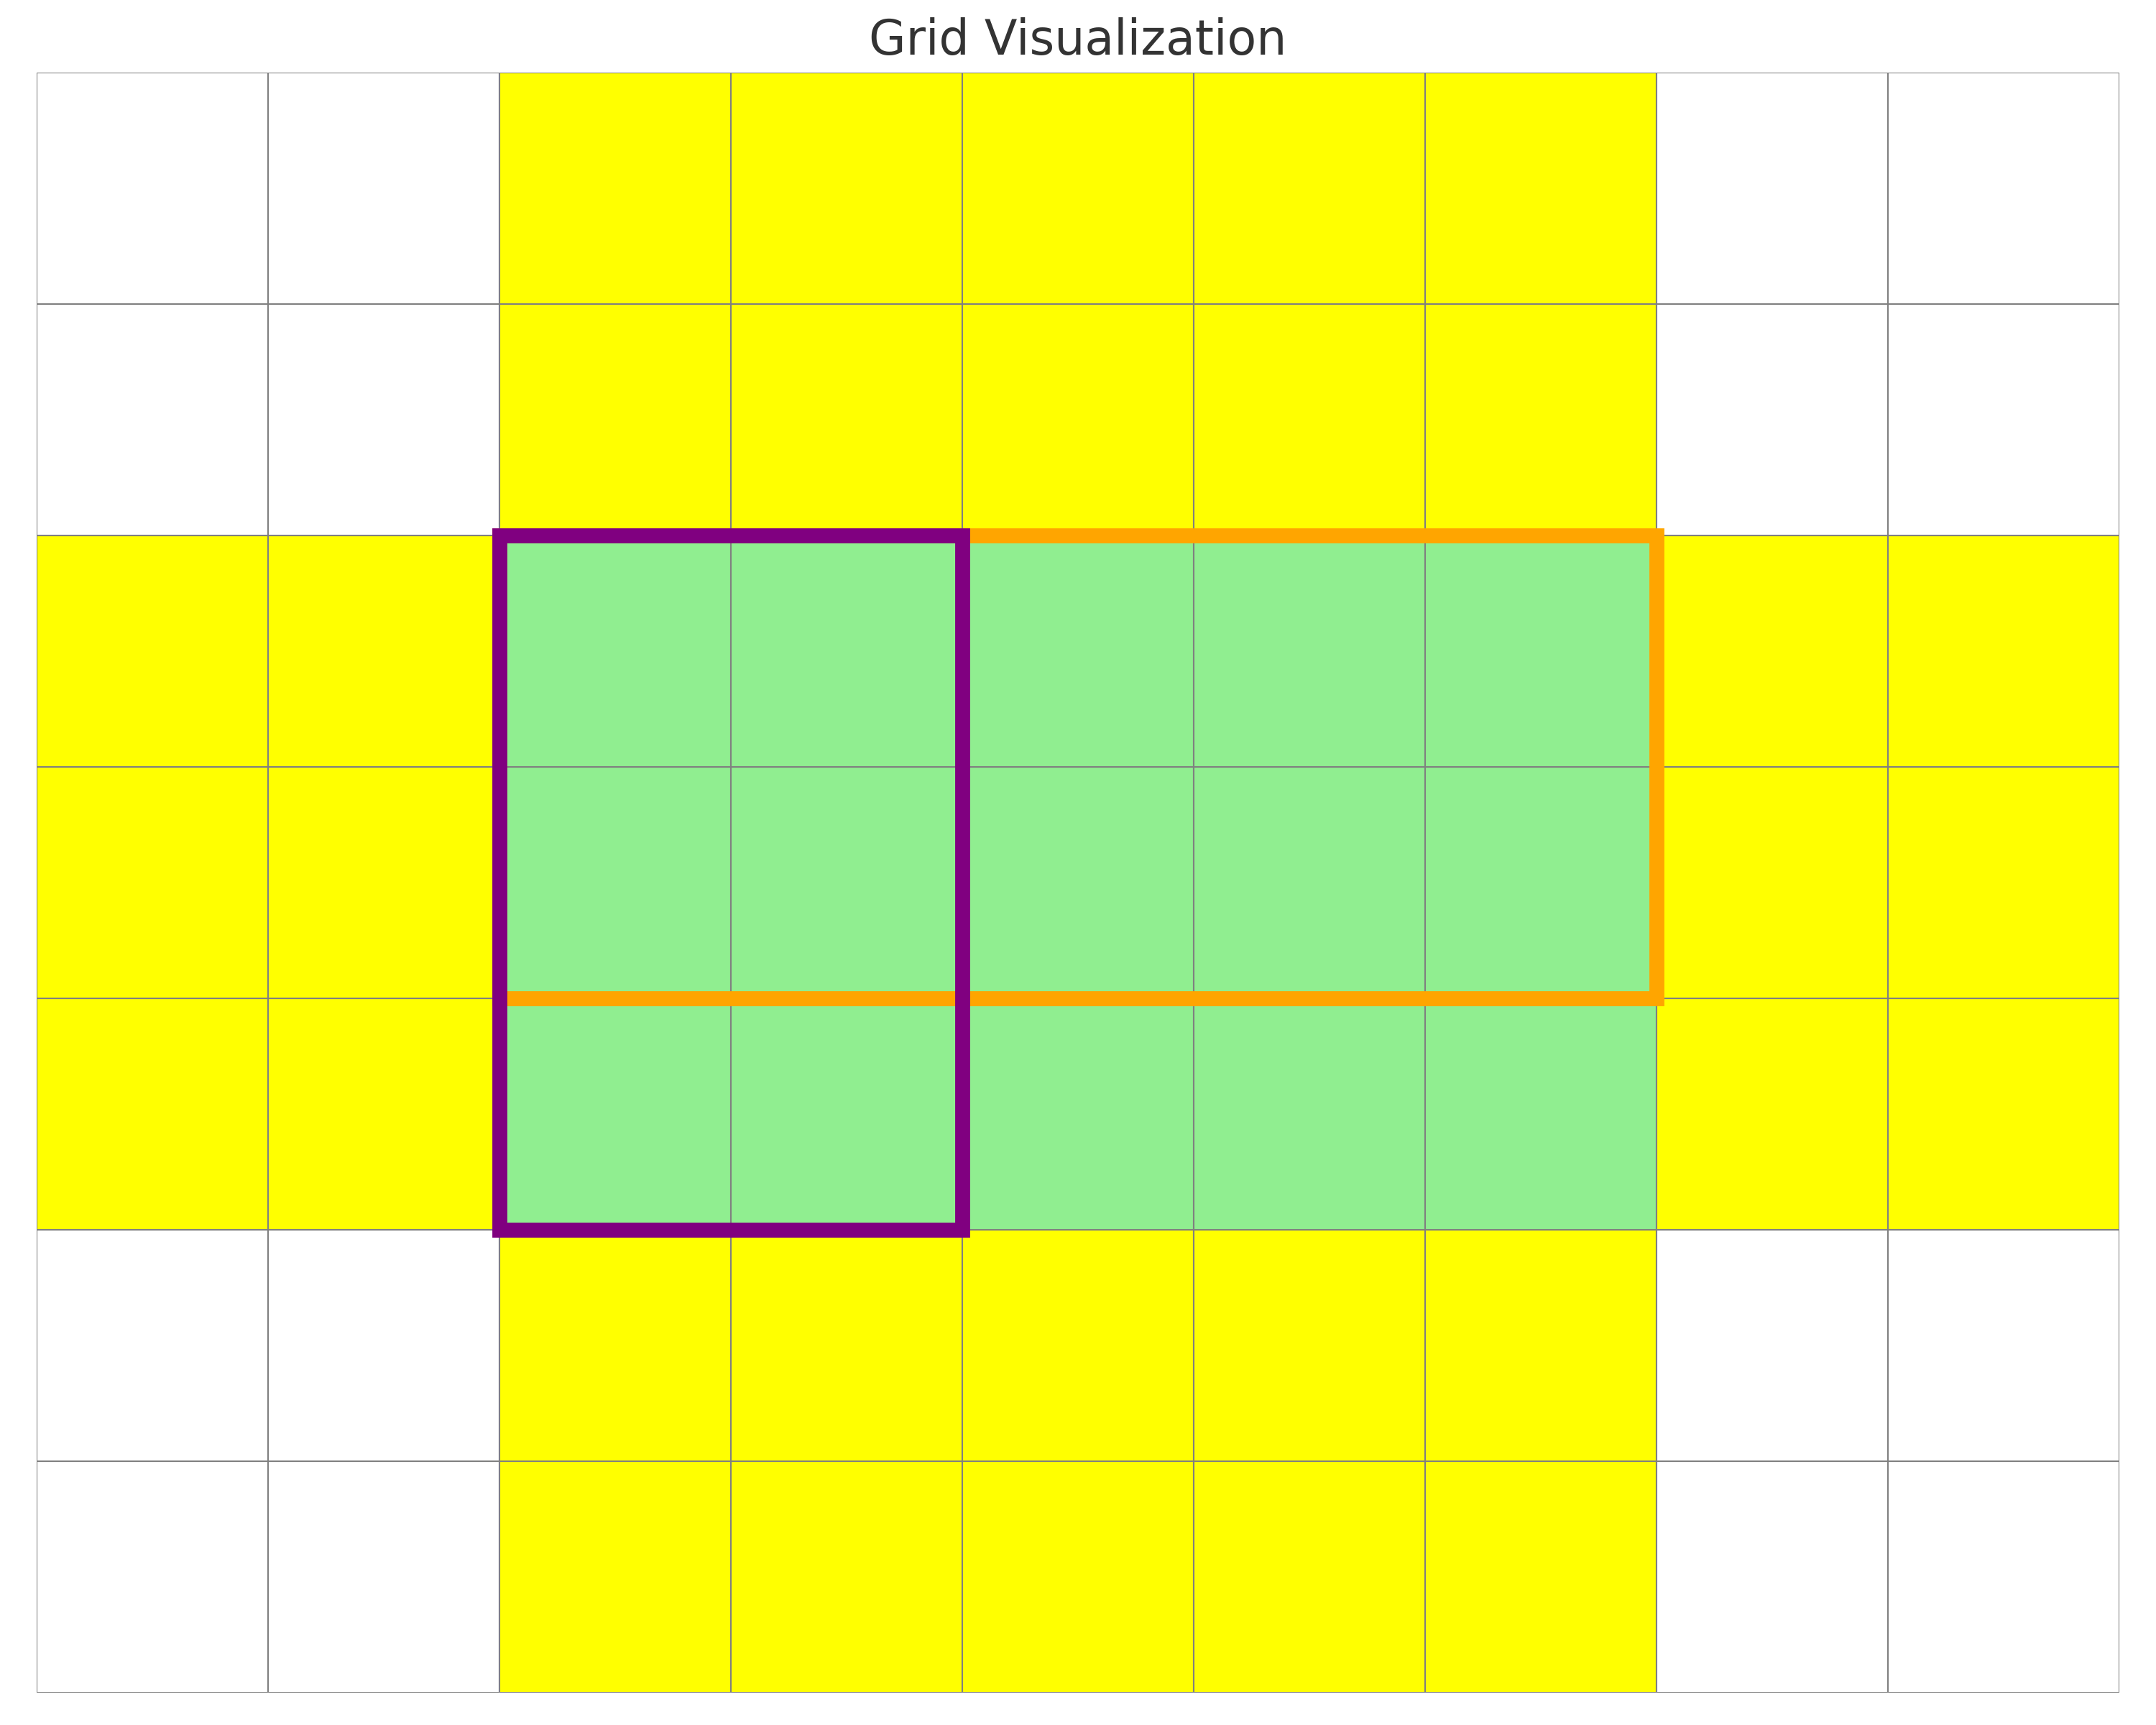
\includegraphics[width=0.5\linewidth]{grid_visualization.png}
    \caption{Data layout within two neighboring \acp{pe} for the tiled stencil with tile size $t_w=3, t_h=4$ and radius $r=2$. The light green area represents the \ac{pe}'s assigned grid tile. The surrounding light blue halo region stores data received from neighbors, while the green and blue thick borders show the data regions exchanged between neighboring \acp{pe}.}
    \label{fig:grid_visualization}
\end{figure}
The communication for the variable tile size requires one \ac{pe} to send different data to its neighbors. This is visualized in \autoref{fig:grid_visualization}. This requires four distinct colors for sending to the different neighbors as well as four colors to receive. For each of the four directions, a pair of colors is used and arranged in a checkerboard pattern across the \ac{pe}-grid.
If colors 0 and 1 are used for data transfer from west to east, following function can be used to determine what color is used to send and to receive:
\begin{equation}
    \label{eq:tiled_coloring_function}
    f(row, col)=(row+col) \bmod 2
\end{equation}
Where $f$ determines the color used to send data east and $1-f$ is used to receive from west. The same method is also applied for the other directions.

\subsection{\ac{pe} Program}

\begin{figure}
    \centering
    \animategraphics[autoplay,loop,controls=false,width=\linewidth]{0.5}{stencil_frames/frame_0}{0}{8}
    \caption{Animation of the computational steps for one iteration of the tiled algorithm with radius $r=2$. Each frame highlights the rectangular region of the buffer being accessed and multiplied by a weight, with the result accumulated. The sequence demonstrates how the algorithm iterates through the halo regions as the values for the next iteration are computed. (Note: Animation may require a compatible PDF viewer).}
    \label{fig:stencil_algorithm_animation}
\end{figure}

The tile of the grid, held by single \ac{pe} is stored in the center region of a 2D array of size $(t_h+2r)\times (t_w+2r)$ - the $buffer$. This array is larger than the tile itself to allow for the halo region, which is used to store the data received from the neighbors. Furthermore an accumulator array of the same size is used to store the intermediate values of the stencil computation. In this array, only the center of size $t_h, t_w$ is used. Choosing its size to be the same as the buffer leads to more consistent memory access patterns, which reduces bank conflicts.

Two \texttt{mem4d\_dsd}s per direction are used for communication. One that specifies the location within the buffer of the data to send and one that specifies the location of the data to receive.
Asynchronous \texttt{@fmovs} instructions are used for data exchange. Two counters track the completion of asynchronous send and receive operations. Once all four neighbor data blocks have been sent and all four have been received, the main computation task is triggered. This ensures that the computation only starts once all necessary data is available in the halo regions.

The \ac{dsd} configuration for the tiled implementation is shown in \autoref{lst:dsd_config}.

\begin{lstlisting}[language=CSL, caption={DSD Configuration for Tiled Implementation}, label={lst:dsd_config}]
    const all_buffer_dsd = @get_dsd(mem4d_dsd, .{ 
        .tensor_access = |i, j|{tile_height + 2*radius, tile_width + 2*radius} 
            -> buffer[i, j] 
    });
    const buffer_center_dsd = @get_dsd(mem4d_dsd, .{ 
        .tensor_access = |i, j|{tile_height, tile_width} 
            -> buffer[radius + i, radius + j] 
    });
    const buffer_send_west_dsd = @get_dsd(mem4d_dsd, .{ 
        .tensor_access = |i, j|{tile_height, radius} 
            -> buffer[i + radius, j + radius] 
    });
    const buffer_send_east_dsd = @get_dsd(mem4d_dsd, .{ 
        .tensor_access = |i, j|{tile_height, radius} 
            -> buffer[i + radius, tile_width + j] 
    });
    const buffer_recv_west_dsd = @get_dsd(mem4d_dsd, .{ 
        .tensor_access = |i, j|{tile_height, radius} 
            -> buffer[radius + i, j] 
    });
    const buffer_recv_east_dsd = @get_dsd(mem4d_dsd, .{ 
        .tensor_access = |i, j|{tile_height, radius} 
            -> buffer[radius + i, tile_width + radius + j] 
    });    
\end{lstlisting}


A \ac{dsd} is used to select the center region of the buffer. This \ac{dsd} is subsequently shifted to represent a rectangular area of the buffer that is shifted up, down, left or right by a number of elements up to the radius from the center. \texttt{@fmacs} instructions are used to multiply these values with the respective weight and add the results to the accumulator. The accumulator is then multiplied with the weight $w_0$ and added to the center region of the buffer to complete the iteration. This process is visualized in \autoref{fig:stencil_algorithm_animation}.

If only \texttt{@fmacs} instructions were used, the accumulator would have to be reset to zero after each iteration. To avoid this, a \texttt{@fmuls} instruction is used for the very first operation that writes to the accumulator to overwrite the values of the previous iteration.

\begin{algorithm}[tbh]
    \SetAlgoLined
    \KwData{Buffer with halo regions filled}
    \KwResult{Updated buffer center}
    \For{$i \gets 1$ \KwTo $r$}{
        \eIf{$i == 1$}{
            $accumulator \gets weights[i] \cdot buffer\_center\_dsd_{UP,i}$\;
        }{
            $accumulator \gets accumulator + weights[i] \cdot buffer\_center\_dsd_{UP,i}$\;
        }
        $accumulator \gets accumulator + weights[i] \cdot buffer\_center\_dsd_{DOWN,i}$\;
        $accumulator \gets accumulator + weights[i] \cdot buffer\_center\_dsd_{LEFT,i}$\;
        $accumulator \gets accumulator + weights[i] \cdot buffer\_center\_dsd_{RIGHT,i}$\;
    }
    $buffer\_center\_dsd \gets buffer\_center\_dsd + weights[0] \cdot accumulator$\;
    \caption{Tiled algorithm code}\label{alg:tiled_algorithm}
\end{algorithm}

The Dirichlet border is implemented by using a ring of \acp{pe} that only send and receive data from their neighbors and do not participate in the computation. If $r<t_w$ or $r<t_h$ the border \acp{pe} values are padded with zeros to fill their buffer. Re refer to the \acp{pe} that only send and receive data from their neighbors as border \acp{pe}, the ones that participate in the computation as inner \acp{pe} and the set of both of these as active \acp{pe}.

\begin{table}[h]
    \centering
    \caption{Operations for one grid point and iteration, tiled implementation with radius $r$}
    \label{tab:tiled_operations}
    \begin{tabular}{@{}cccc@{}}
        \toprule
        Operation & Cerebras Op Code & Count & Flops \\
        \midrule
        fmac & \texttt{@fmacs} & $5r-1$ & $10r-2$ \\
        mul & \texttt{@fmuls} & \num{1} & \num{1} \\
        \midrule
        total & & $5r$ & $10r-1$ \\
        \bottomrule
    \end{tabular}
\end{table}

\subsection{r1-optimized version}

As a special case of the tiled algorithm, the problem with radius one was further optimized by using \texttt{mem1d\_dsd}s instead of \texttt{mem4d\_dsd}s for the halo regions where the neighbors data is received as well as the data to send. Furthermore the shifted \acp{dsd} are precomputed and all \acp{dsd} are explicitly assigned to distinct \acp{dsr}. There are enough \acp{dsr} available so that each \ac{dsr} is used for at most one \ac{dsd}. This allows for a significant reduction in the number of cycles per iteration, since loading the \acp{dsd} into \acp{dsr} only needs to be done once, independent of the number of iterations. We still find that the \acp{dsd} used for reading the parts of the buffer that are send to the neighbors and the ones describing the halo regions for receiving need to be reloaded to the \acp{dsr} for each iteration. The load to \ac{dsr} for these \acp{dsd} acts as a kind of reset and if not done, it leads to buffer overflows. The documentation doesn't specify this requirement and interestingly, it is not necessary for all \acp{dsd}. 
As another optimization, \texttt{@fadds} are used instead of \texttt{@fmacs} and the multiplication is handled separately. This reduces the flop number from $9$ to $6$ per element and results in a performance improvement because the simd width for \texttt{@fadds} is 2/4 on wse-2/3 while it is only 1 for \texttt{@fmacs}. Note that the shifted \acp{dsd} $buffer\_center\_dsd_{DIR,i}$ in the general version need to be created for each iteration of the loop while pre-computed \acp{dsd} are used in this optimized version.
Furthermore we find that on \ac{wse}-3 for radius one and tile sizes greater than four, we can rely on explicitly set task priorities instead of counters to ensure the computation task only starts if all data is receive. This further reduces overhead. 

For all experiments in this work, the r1-optimized version is used whenever applicable, except when explicitly stated otherwise.

\begin{algorithm}[tbh]
    \SetAlgoLined
    \KwData{Buffer with halo regions filled}
    \KwResult{Updated buffer center}
    $accumulator \gets buffer\_center\_dsd \cdot weights[0]/weights[1]$\;
    $accumulator \gets accumulator + buffer\_center\_dsd_{UP,1}$\;
    $accumulator \gets accumulator + buffer\_center\_dsd_{DOWN,1}$\;
    $accumulator \gets accumulator + buffer\_center\_dsd_{LEFT,1}$\;
    $accumulator \gets accumulator + buffer\_center\_dsd_{RIGHT,1}$\;
    $buffer\_center\_dsd \gets buffer\_center\_dsd + accumulator \cdot weights[1]$\;
    \caption{Radius-1, tiled algorithm code}\label{alg:r1_tiled_algorithm}
\end{algorithm}

\begin{table}[h]
    \centering
    \caption{Operations for one grid point and iteration, r1 optimized tiled implementation}
    \label{tab:tiled_operations_r1_optimized}
    \begin{tabular}{@{}cccc@{}}
        \toprule
        Operation & Cerebras Op Code & Count & Flops \\
        \midrule
        add & \texttt{@fadds} & \num{4} & \num{4} \\
        mul & \texttt{@fmuls} & \num{2} & \num{2} \\
        \midrule
        total & & \num{6} & \num{6} \\
        \bottomrule
    \end{tabular}
\end{table}

Our implementation is open source and available at \url{https://github.com/Jorineg/cerebras}
